\documentclass[11pt,a4paper]{ctexart}

\usepackage{amsmath}
\usepackage{amssymb}
\usepackage{array}
\usepackage{booktabs}
\usepackage{geometry}
\usepackage{graphicx}
\usepackage{hyperref}

%% Script:  analysis-3/code/analysis-3.py
%% Outputs: analysis-3/code/analysis-3_*.{json,csv}
%% Figures: analysis-3/figures/

\geometry{left=2.4cm,right=2.4cm,top=2.4cm,bottom=2.4cm}
\graphicspath{{figures/}}

\title{Pre-Analysis 3\\[4pt]
\large rooted-shell 刺激分类与 \texorpdfstring{$\rho$}{rho}-separability}
\author{}
\date{\today}

\begin{document}
\maketitle

\tableofcontents
\bigskip

\section{执行目标}

本分析对应 `TODO-3.md`，目标不是再回答“5 节点还是 6 节点更好”，而是把 stimulus design 重新表述为以目标节点 $X$ 为中心的 rooted-shell 结构问题。核心问题是：
\begin{quote}
哪些 rooted structural dimensions 决定了 $M_0 \rightarrow M_\rho \rightarrow M_\mathrm{exact}$ 的可分离性？
\end{quote}

因此，本分析把 node count 降为实现某个 rooted motif 的最小容器，而把真正的科学变量固定为 3 个维度：
\begin{enumerate}
    \item D1: target degree $|S_1|$
    \item D2: shell-1 内部耦合 $e_{11}$
    \item D3: remote structure（用 $|S_2|, e_{12}, e_{22}$ 细化）
\end{enumerate}

另外，analysis-2 已经证明 adaptive conflicting evidence 优于 uniform 设计，因此 TODO-3 中 evidence strategy 固定为该 winning design，不再重新比较。

\section{方法}

\subsection{rooted 图目录}

我们枚举了 $n=5,6$ 上所有 connected、3-colorable 的图，并以目标节点 $X$ 为中心做 rooted 去重：若同一无根图有多个 graph center，则保留所有互不等价的 rooted-canonical 形式。最终得到
\[
200
\]
个 rooted graph motifs，其中：
\begin{itemize}
    \item $n=5$：27 个 rooted motifs
    \item $n=6$：173 个 rooted motifs
\end{itemize}

这里的结论不是“6 节点更重要”，而是“6 节点提供了更多可分离的 rooted motifs”。node count 只是容器，真正的解释变量来自 rooted descriptor。

\subsection{三维 rooted-shell descriptor}

对于每个 rooted graph，我们记录：
\[
S_1 = N(X),
\qquad
S_2 = \{v : d_G(X,v)=2\}.
\]

并进一步记录：
\[
|S_1|,
\qquad
 e_{11},
\qquad
 |S_2|,
\qquad
 e_{12},
\qquad
 e_{22}.
\]

在报告层面，远端结构 D3 被编码成三类：
\begin{itemize}
    \item D3-0: no remote structure ($|S_2|=0$)
    \item D3-1: tree-like remote structure ($|S_2|>0$, $e_{12}=|S_2|$, $e_{22}=0$)
    \item D3-2: strong remote structure（其余所有有远端结构的情形）
\end{itemize}

这个编码方式的直观含义是：D3-1 只是在 immediate neighbourhood 外再接出一层树枝，而 D3-2 则包含多重回连或远端闭合结构。

\subsection{rho-agent 计算}

延续 analysis-2，所有预测都使用精确穷举：
\begin{itemize}
    \item 5 个代理：$\rho = 0, 0.25, 0.5, 0.75, 1$
    \item 能量衰减形式：
    \[
    \psi^{(\rho)}_{uv}(x_u,x_v)
    =
    \exp\!\left[-\beta_{\mathrm{edge}}\,\rho^{s(u,v)}\,\mathbf{1}(x_u=x_v)\right]
    \]
    \item $\beta_{\mathrm{edge}} = 4$
    \item brute-force exact summation only
\end{itemize}

对每个 rooted graph，固定使用 adaptive conflicting evidence 选出的最佳 evidence template，然后记录：
\begin{itemize}
    \item $D_{\mathrm{KL}}(\tilde b_0 \| \tilde b_1)$ under high evidence
    \item 相邻 $\rho$ 水平 KL 总和
    \item $p_R$ 与 $H(\tilde b_\rho)$ 的单调性
\end{itemize}

\section{结果 1：descriptor framing 比 node-count framing 更有解释力}

先看 node count 的粗略分组：

\begin{table}[ht]
\centering
\small
\begin{tabular}{lcccc}
\toprule
node count & rooted motifs & mean $D_{\mathrm{KL}}(\tilde b_0 \| \tilde b_1)$ & min & max \\
\midrule
$n=5$ & 27 & 0.334 & 0.000 & 1.038 \\
$n=6$ & 173 & 0.632 & 0.000 & 1.880 \\
\bottomrule
\end{tabular}
\caption{按 node count 分组的 separability。这个分组过于粗糙：同一个 $n$ 内部的差异范围很大，因此无法解释哪类 rooted motif 真正有区分力。}
\end{table}

相比之下，按 D3 分组得到一个更清楚的有序梯度：

\begin{table}[ht]
\centering
\small
\begin{tabular}{lcccc}
\toprule
D3 class & rooted motifs & mean $D_{\mathrm{KL}}(\tilde b_0 \| \tilde b_1)$ & min & max \\
\midrule
D3-0: no remote & 20 & 0.225 & 0.000 & 0.348 \\
D3-1: tree-like remote & 32 & 0.461 & 0.112 & 1.054 \\
D3-2: strong remote & 148 & 0.670 & 0.003 & 1.880 \\
\bottomrule
\end{tabular}
\caption{按 rooted remote-structure class 分组的 separability。与 raw node count 相比，D3 更直接地刻画了何时远端结构会真正影响目标后验。}
\end{table}

这就是 TODO-3 的核心结果：\textbf{真正有解释力的不是图有几个点，而是远端结构是否存在、以及它如何回连到第一层邻域。}

完整 rooted taxonomy 共得到：
\begin{itemize}
    \item 32 个 main descriptor families（按 D1/D2/D3）
    \item 98 个 raw descriptor classes（按 $|S_1|, e_{11}, |S_2|, e_{12}, e_{22}, \mathrm{radius}$）
\end{itemize}

\begin{figure}[ht]
\centering
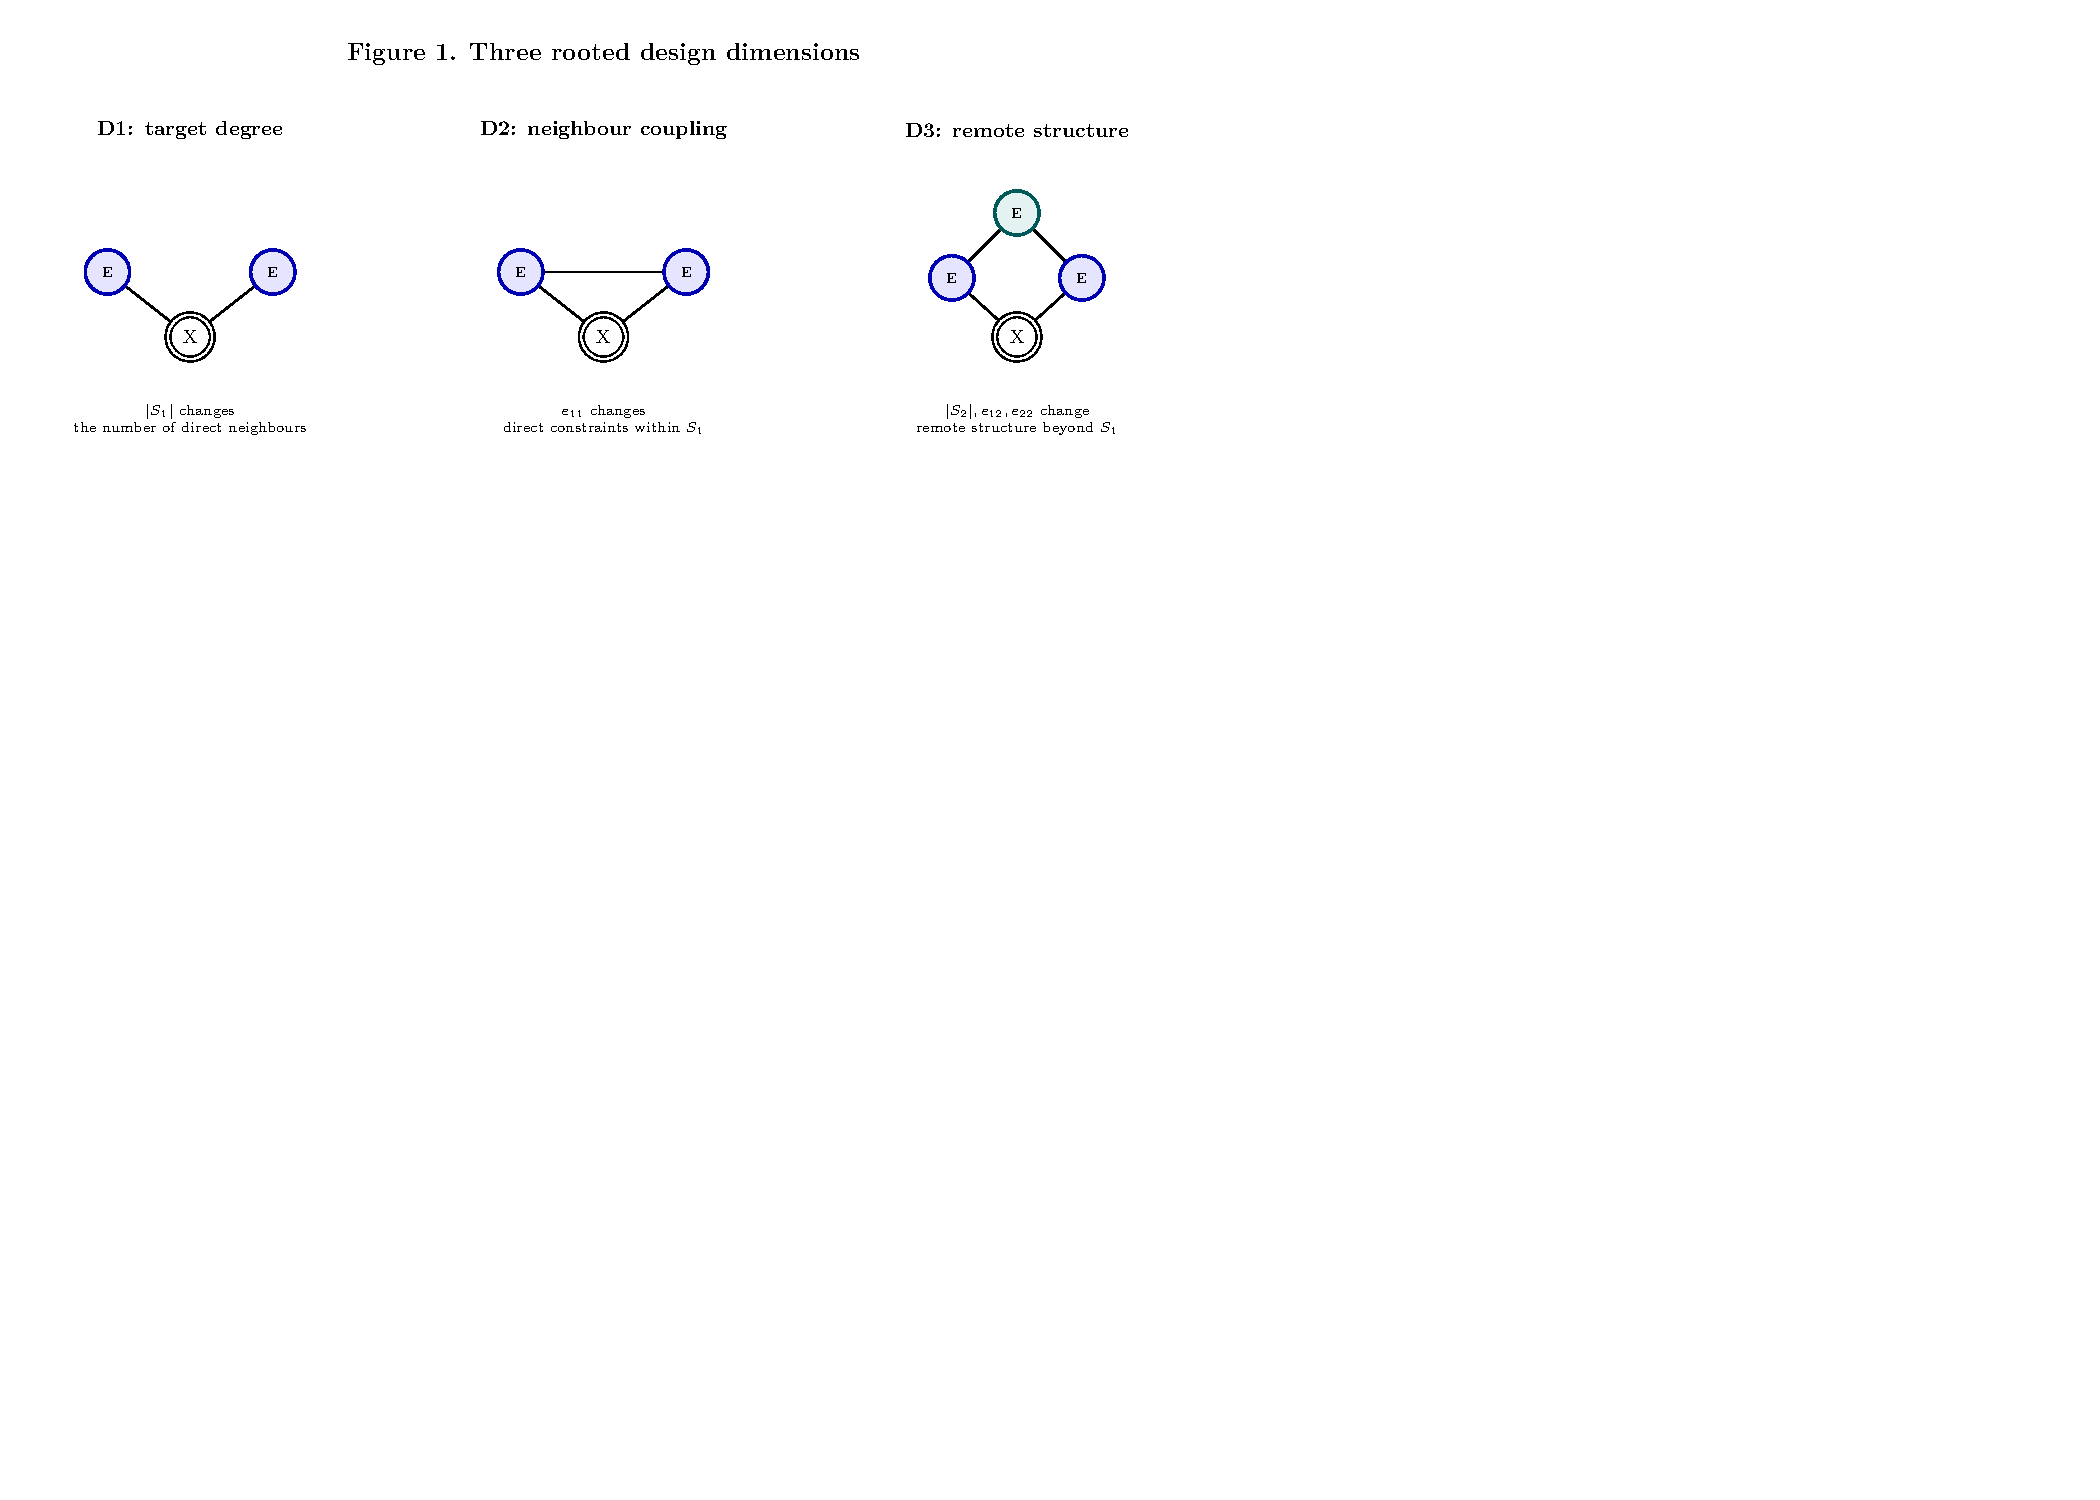
\includegraphics[width=0.95\textwidth]{analysis-3_fig1_design_schematic.pdf}
\caption{Figure 1. rooted stimulus design 的三维示意图。此后刺激不再按 node count，而按 D1 / D2 / D3 组织。}
\end{figure}

\begin{figure}[p]
\centering
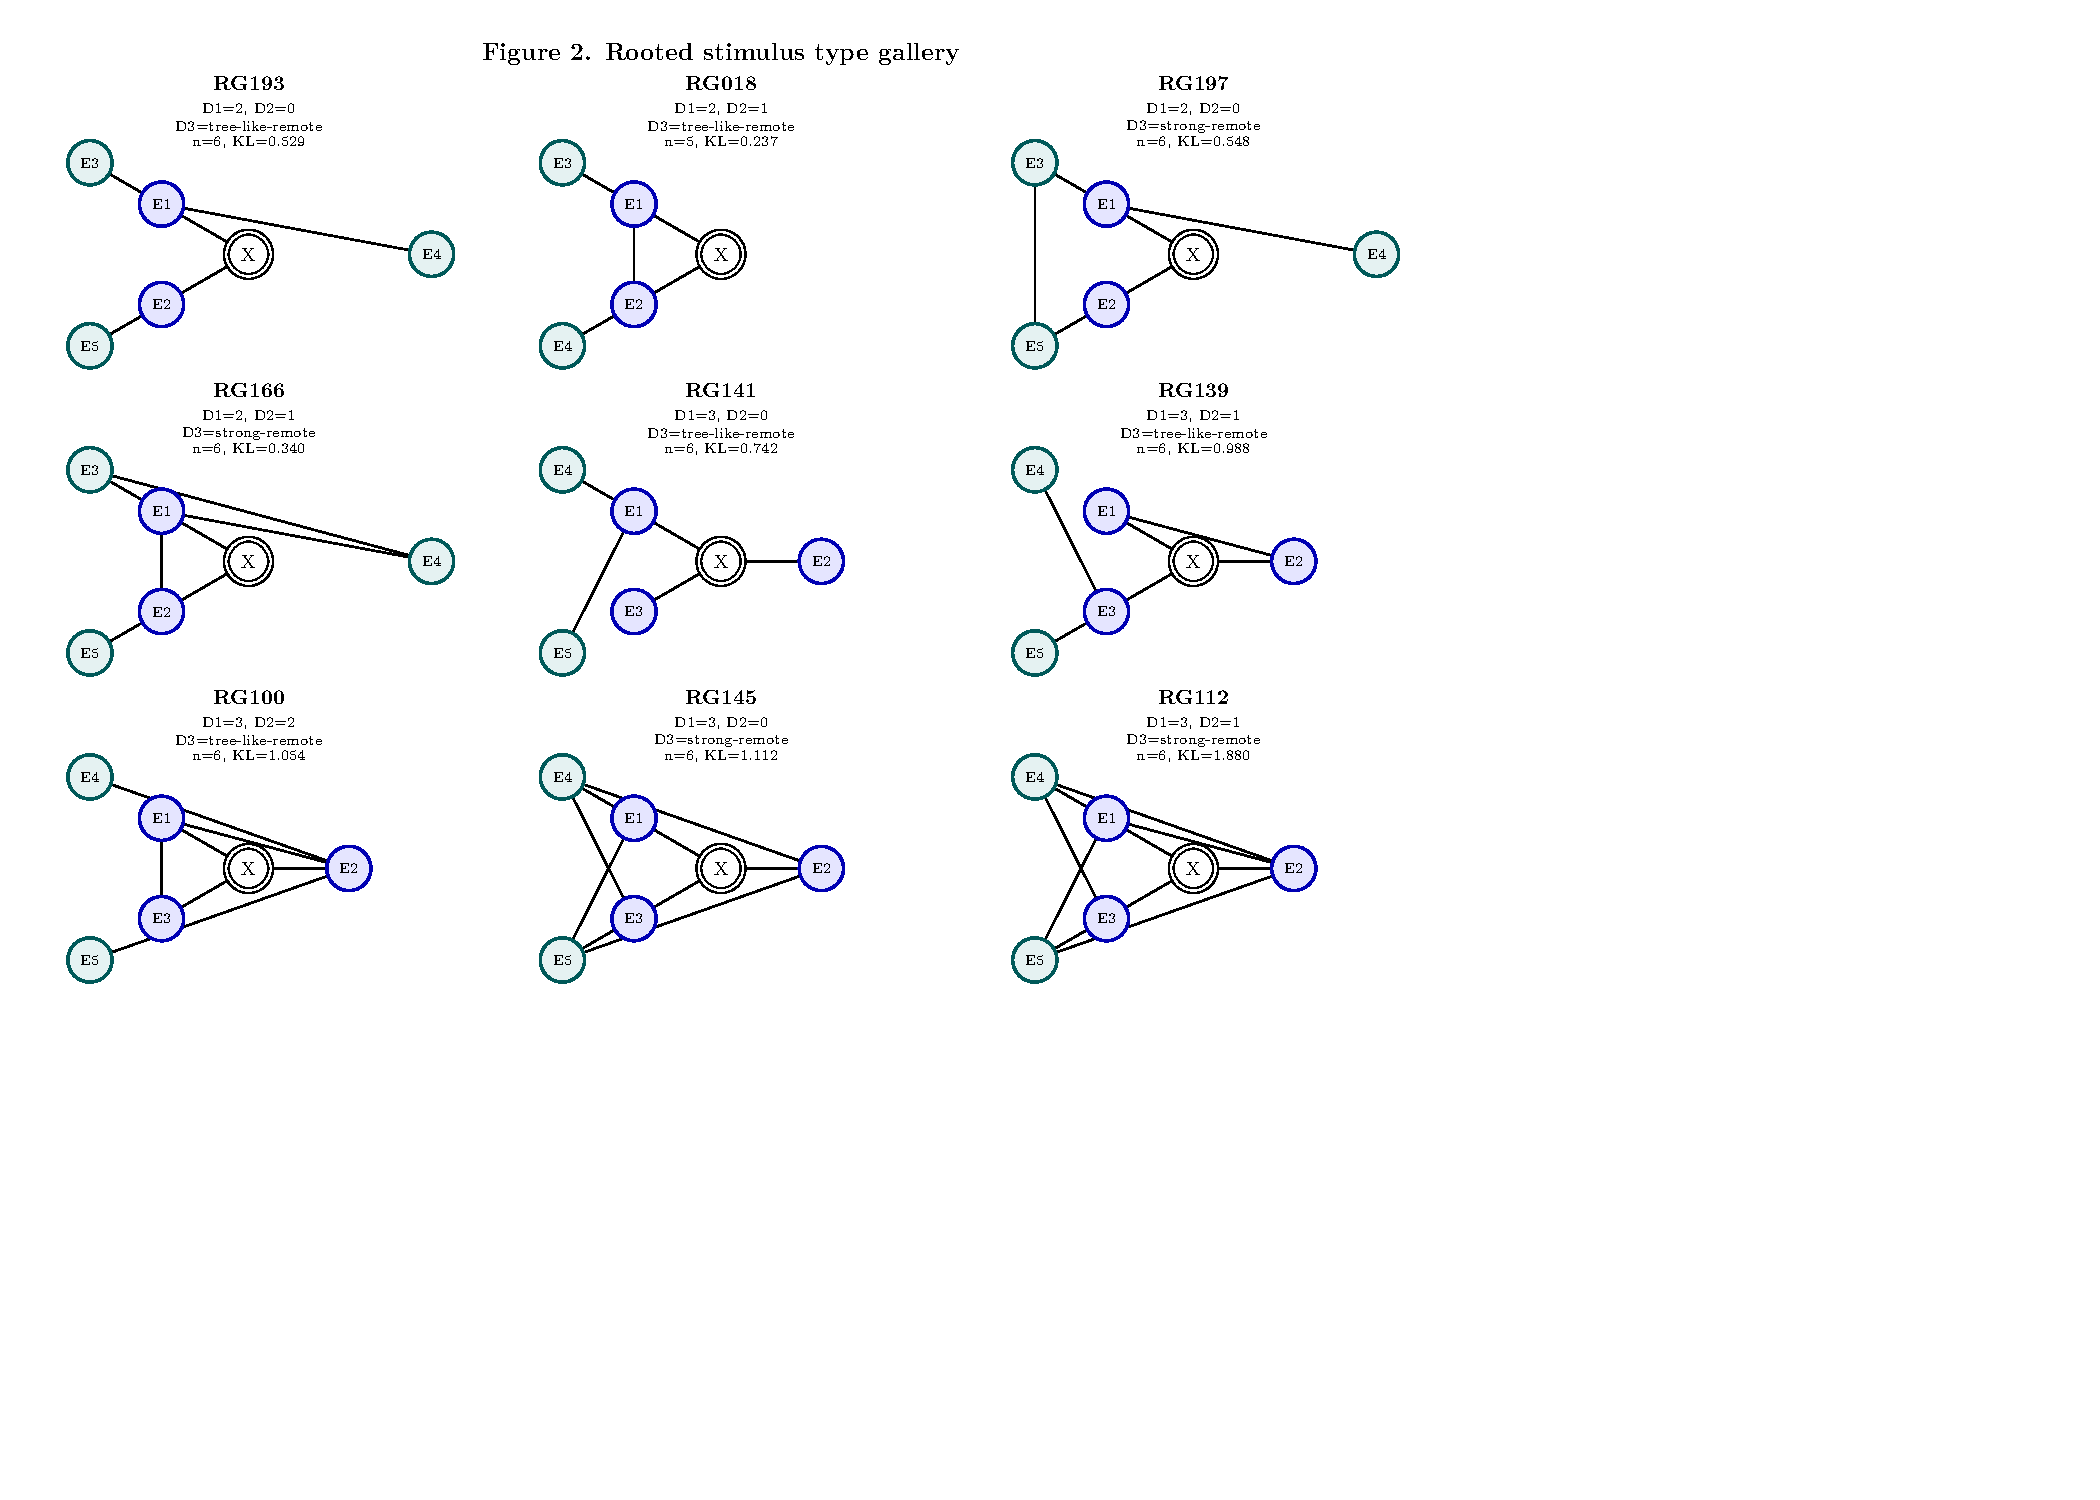
\includegraphics[width=0.97\textwidth]{analysis-3_fig2_rooted_stimulus_gallery.pdf}
\caption{Figure 2. rooted stimulus type gallery。每个小图给出一个 rooted motif exemplar，并标注其 descriptor family 与对应的 high-evidence separability。}
\end{figure}

\clearpage
\section{结果 2：三个维度都能构造成 matched comparison}

TODO-3 要求至少为 D1 / D2 / D3 各找到一个 matched comparison family。结果如下。

\subsection{D1：target degree effect}

最佳 D1 comparison 为 `RG018` 与 `RG139`：
\begin{itemize}
    \item 两图都满足 D2 = 1
    \item 两图都满足 D3 = tree-like remote
    \item 原始远端 descriptor 也完全匹配：$|S_2|=2$, $e_{12}=2$, $e_{22}=0$
    \item 唯一变化是 D1：$|S_1|$ 从 2 增加到 3
\end{itemize}

对应的 high-evidence separability 从
\[
0.237 \rightarrow 0.988
\]
显著增加。

\subsection{D2：neighbour-neighbour coupling effect}

最佳 D2 comparison 为 `RG088` 与 `RG144`：
\begin{itemize}
    \item 两图都满足 D1 = 3
    \item 两图都满足 D3 = strong remote
    \item 原始远端 descriptor 完全一致：$|S_2|=2$, $e_{12}=5$, $e_{22}=0$
    \item 两图的 adaptive-conflicting evidence template 也一致
    \item 唯一变化是 D2：$e_{11}$ 从 0 变到 2
\end{itemize}

对应的 high-evidence separability 为：
\[
1.093 \rightarrow 1.823.
\]
这说明在强远端结构存在时，单独操纵 shell-1 内部闭合程度，已经足以产生清晰可见的 separability change。

\subsection{D3：remote structure effect}

最佳 D3 comparison 为 `RG003` 与 `RG058`：
\begin{itemize}
    \item 两图都满足 D1 = 4
    \item 两图都满足 D2 = 2
    \item 只改变 D3：从 no-remote 变成 strong-remote
\end{itemize}

对应的 high-evidence separability 从
\[
0.132 \rightarrow 1.030
\]
跃迁式提升。这是 analysis-1 / analysis-2 的 equal-local, distinct-remote 逻辑在 descriptor framing 下的直接推广。

\begin{figure}[p]
\centering
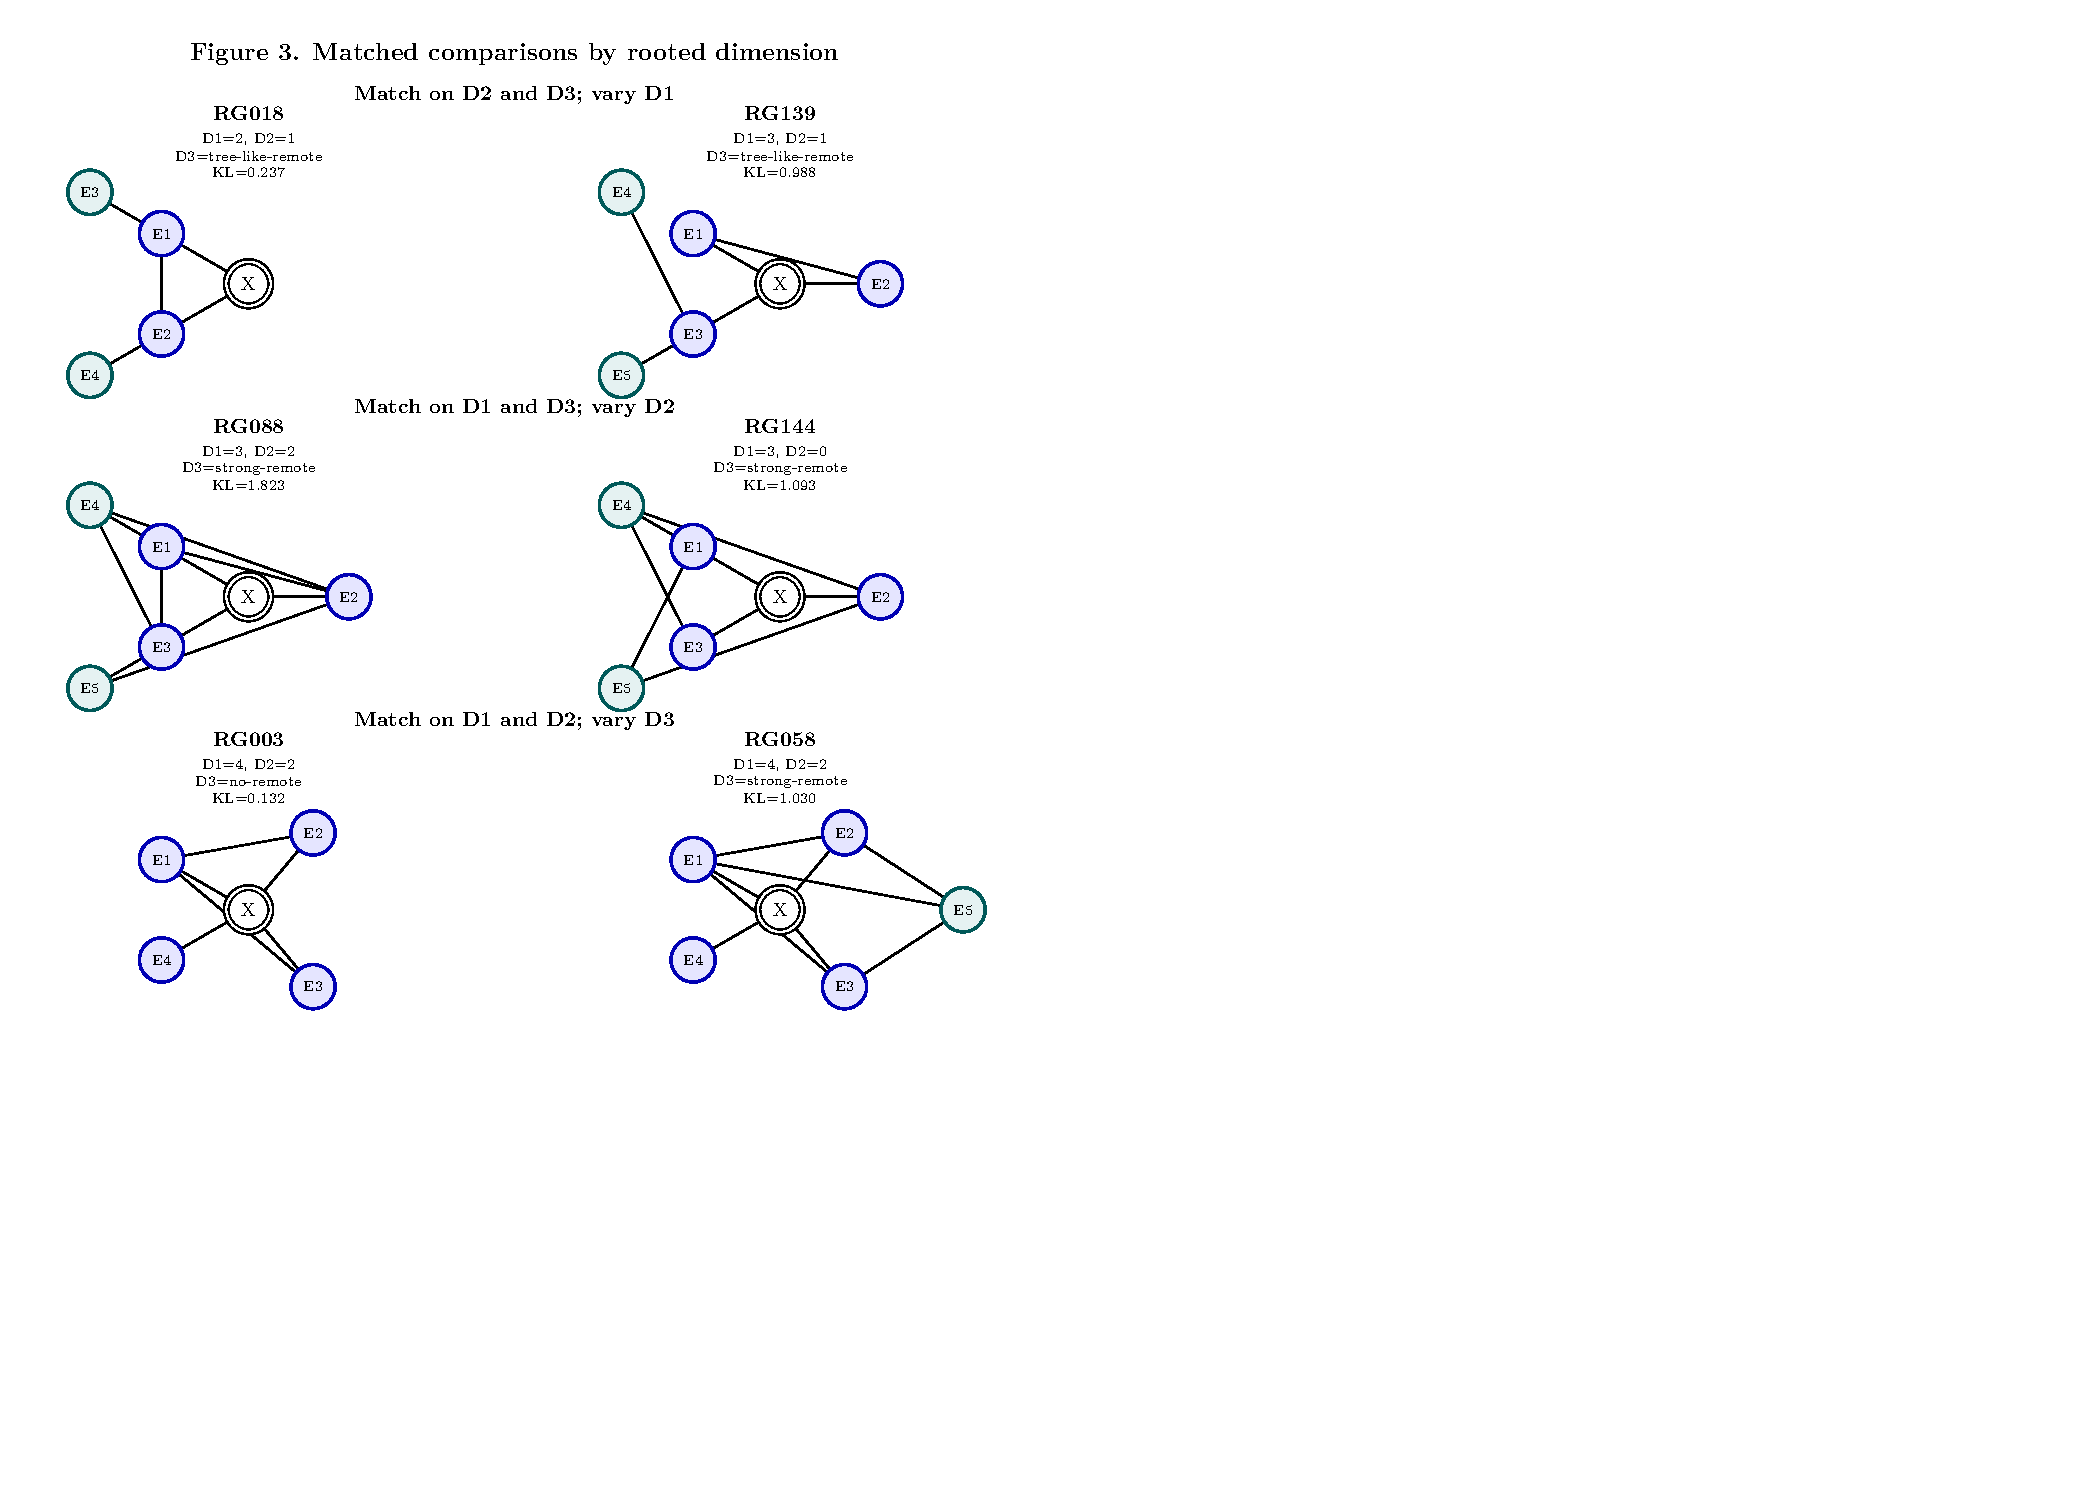
\includegraphics[width=0.97\textwidth]{analysis-3_fig3_matched_comparisons.pdf}
\caption{Figure 3. D1 / D2 / D3 的 matched comparison panels。每一行固定其余维度，只操纵一个目标维度，并在图下标出该 stimulus 的 high-evidence separability。}
\end{figure}

\section{结果 3：候选实验刺激集}

基于 matched comparisons 与高 separability motifs，我们选择了 8 个 candidate stimuli：
\begin{center}
`RG003`, `RG018`, `RG058`, `RG088`, `RG112`, `RG114`, `RG139`, `RG144`
\end{center}

该集合满足：
\begin{itemize}
    \item 覆盖全部 3 个 D3 class
    \item 覆盖 D1 = 2, 3, 4
    \item 覆盖低 / 中 / 高 D2 水平
    \item 含 D1 / D2 / D3 三类 matched comparison 所需图形
    \item 所有图在 high evidence 下都具有非零且清晰的 separability
\end{itemize}

\begin{table}[ht]
\centering
\small
\begin{tabular}{lcccccl}
\toprule
Graph & $n$ & D1 & D2 & D3 & high KL & Reason \\
\midrule
RG003 & 5 & 4 & 2 & no-remote & 0.132 & matched D3 \\
RG018 & 5 & 2 & 1 & tree-like & 0.237 & matched D1 \\
RG058 & 6 & 4 & 2 & strong & 1.030 & matched D3 \\
RG088 & 6 & 3 & 2 & strong & 1.823 & matched D2 \\
RG112 & 6 & 3 & 1 & strong & 1.880 & high separability \\
RG114 & 6 & 3 & 1 & strong & 1.771 & high separability \\
RG139 & 6 & 3 & 1 & tree-like & 0.988 & matched D1 \\
RG144 & 6 & 3 & 0 & strong & 1.093 & matched D2 \\
\bottomrule
\end{tabular}
\caption{最终候选刺激集。Reason 列给出该图被纳入 stimulus set 的主要原因。}
\end{table}

\begin{figure}[p]
\centering
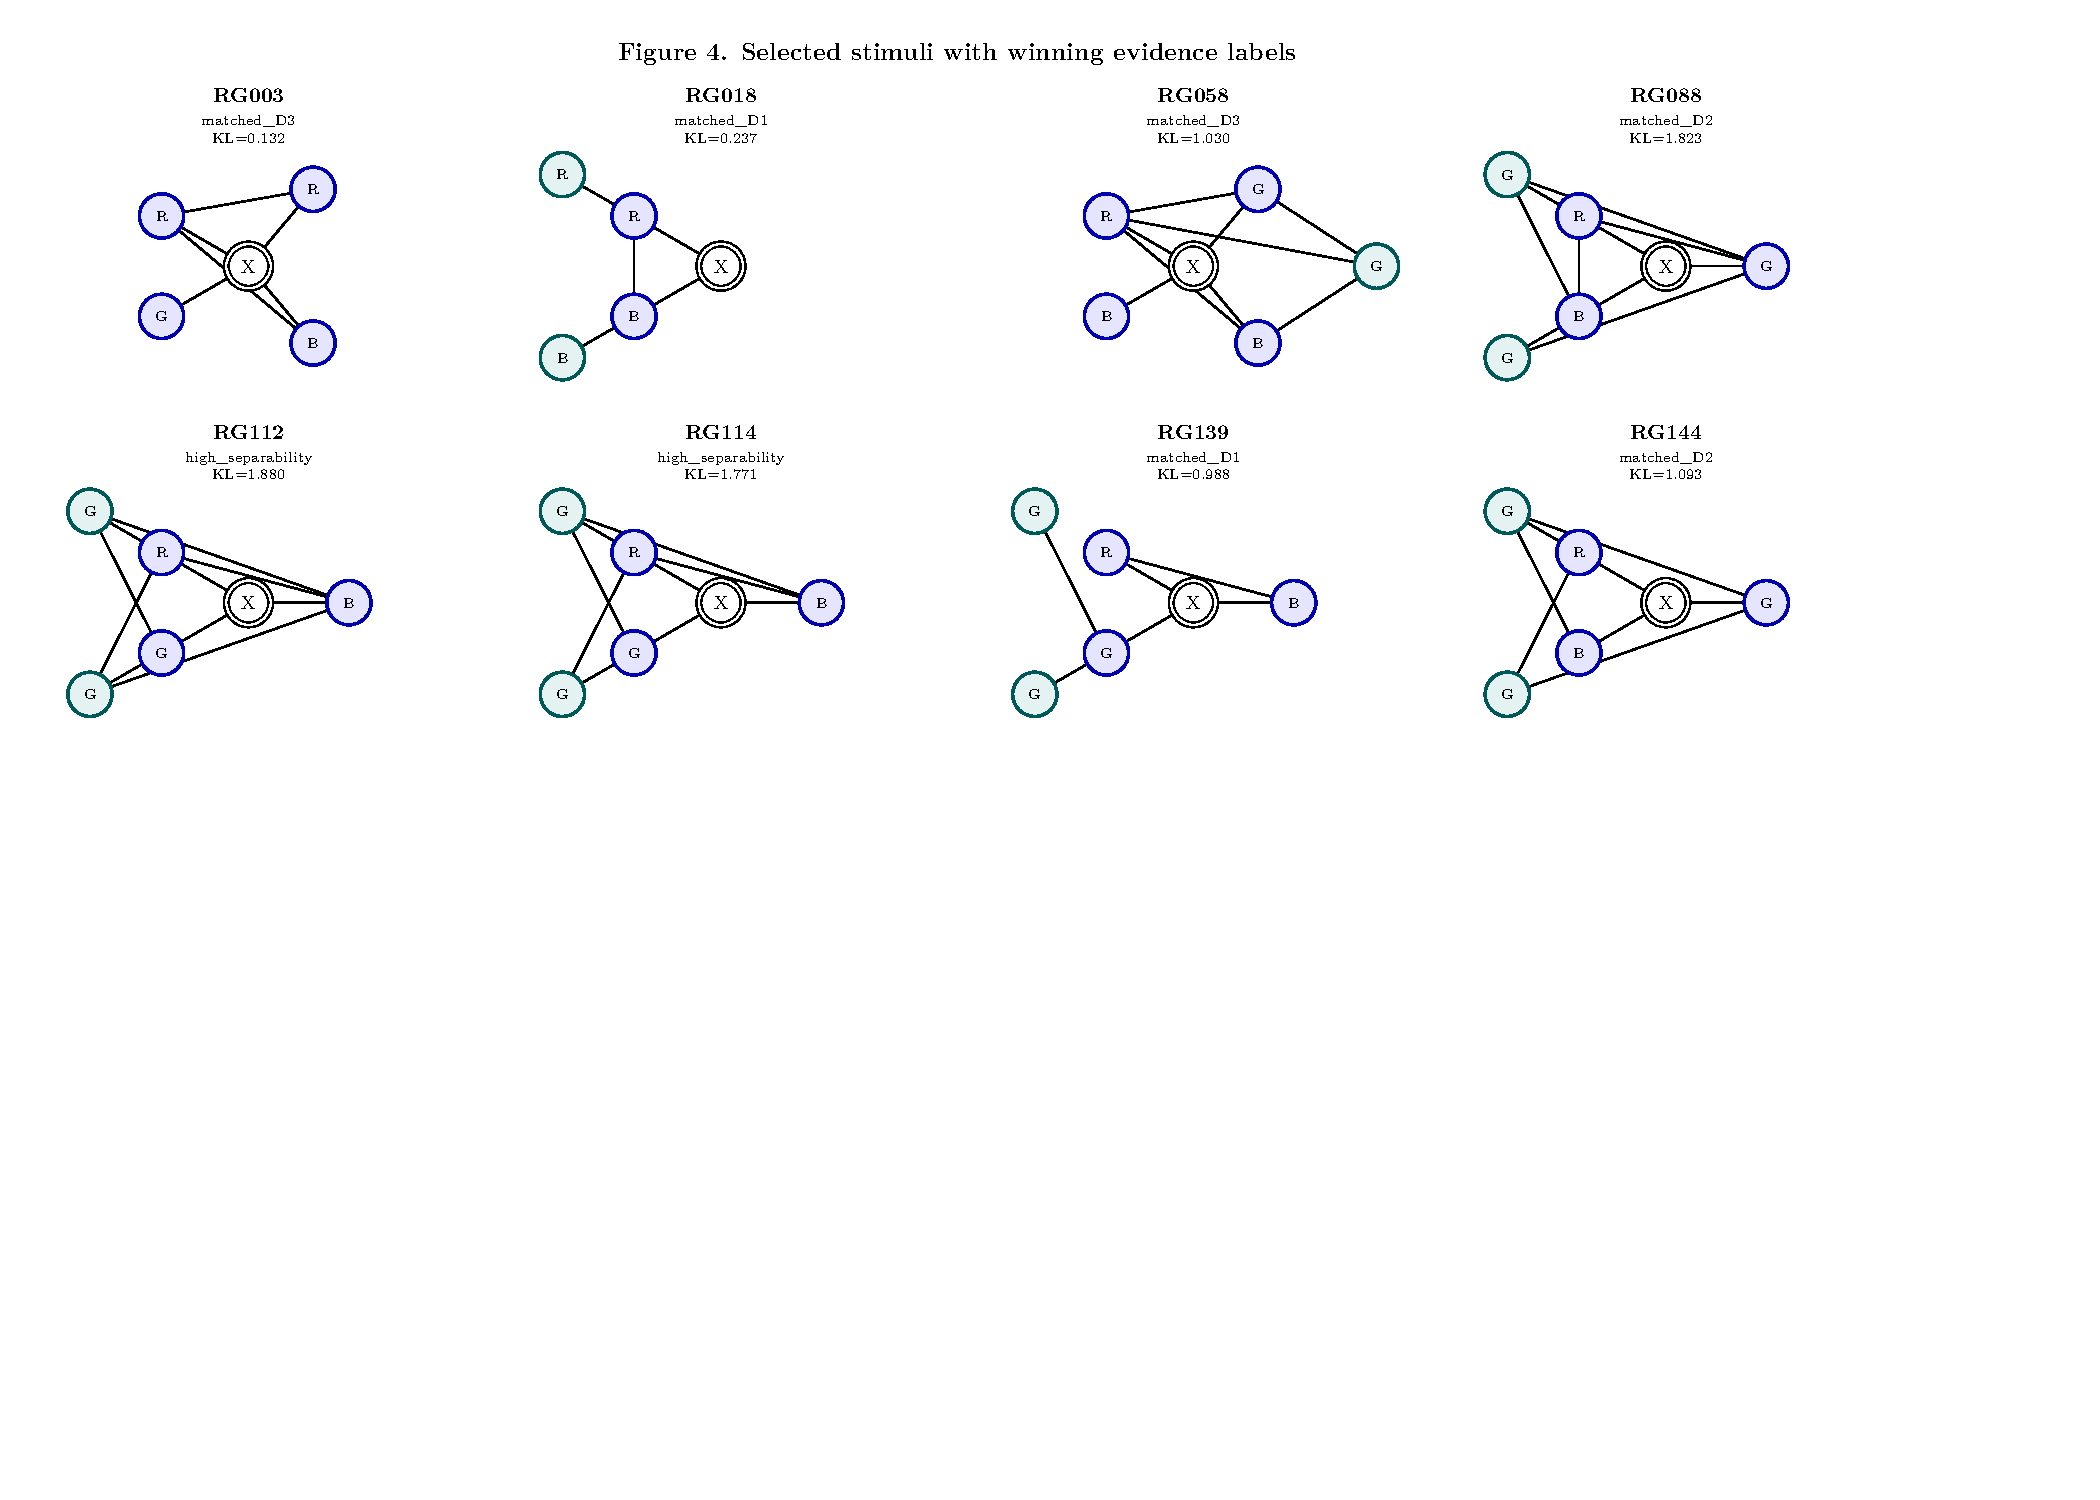
\includegraphics[width=0.97\textwidth]{analysis-3_fig4_selected_stimuli_with_evidence.pdf}
\caption{Figure 4. 最终候选 stimulus set，并直接在节点上标出 adaptive-conflicting strategy 选出的最佳 evidence label（R/G/B）。该图可以直接作为后续实验界面设计的示意基础。}
\end{figure}

\begin{figure}[ht]
\centering
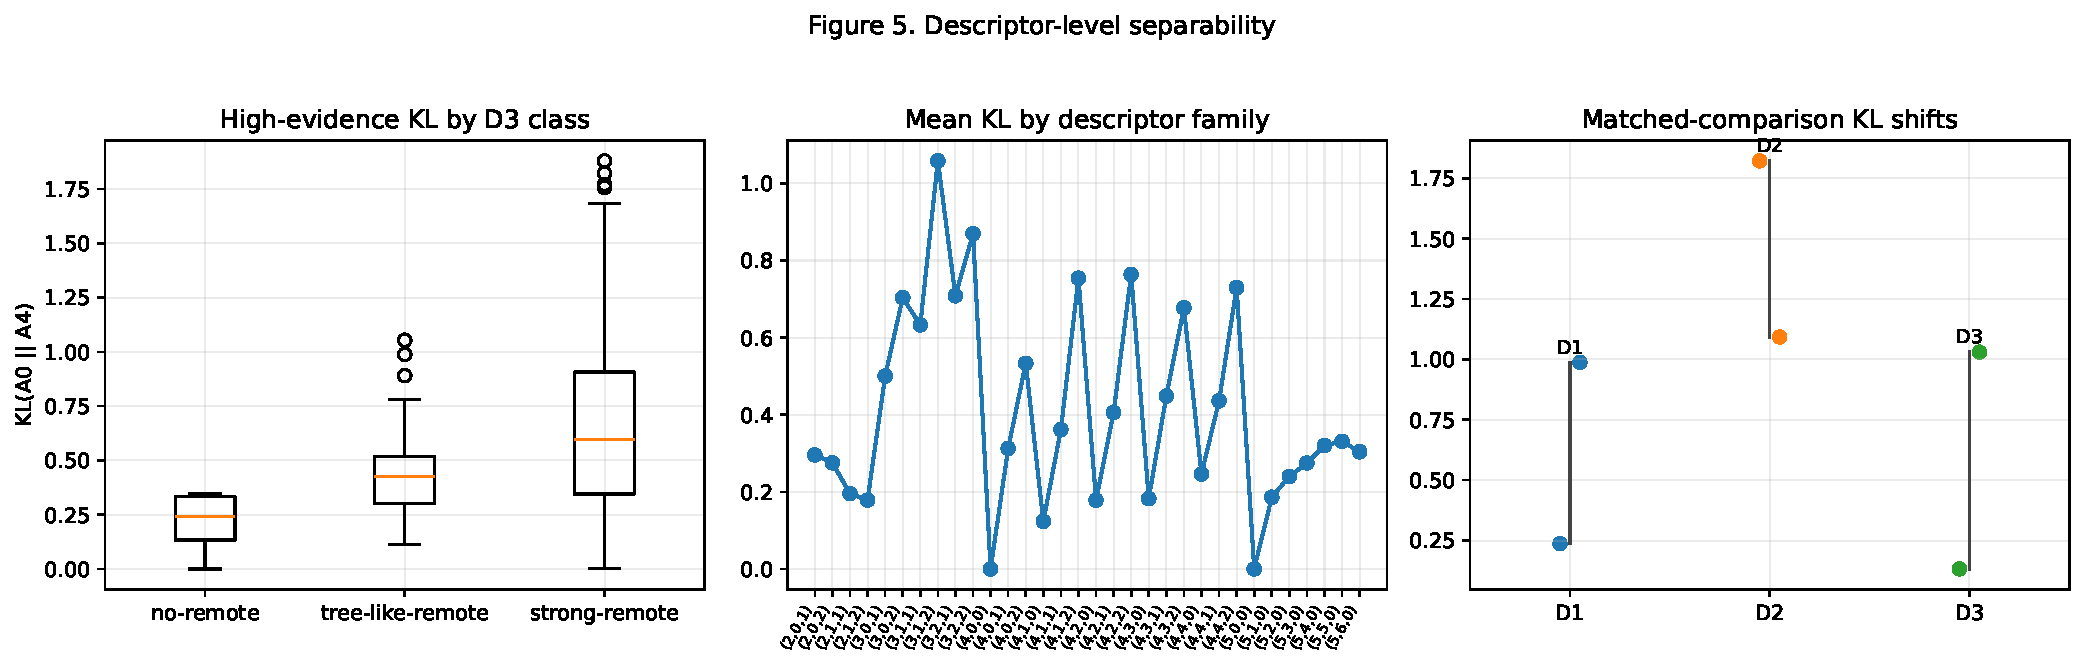
\includegraphics[width=0.98\textwidth]{analysis-3_fig5_descriptor_effects.pdf}
\caption{Figure 5. descriptor-level separability summary。左图显示 D3 class 的有序梯度；中图显示 descriptor family 的平均 separability；右图显示 D1 / D2 / D3 三类 matched comparison 的数值变化。}
\end{figure}

\section{结论}

TODO-3 的 4 条成功标准全部满足：
\begin{enumerate}
    \item \textbf{S1 成功：} rooted descriptor framing 比 raw node count 更有解释力。node count 只能粗略区分平均值，而 D3 class 给出了更稳定、更有结构意义的 separability 梯度。
    \item \textbf{S2 成功：} D1 / D2 / D3 三个维度都构造出了数值上可用的 matched comparison。
    \item \textbf{S3 成功：} 产生了 rooted stimulus taxonomy（32 个 main families, 98 个 raw classes）以及一个可用于后续设计的 candidate stimulus set。
    \item \textbf{S4 成功：} 已经生成 TikZ stimulus sketches，并把 selected stimuli 的 winning evidence template 直接可视化。
\end{enumerate}

科学上的主结论是：
\begin{quote}
\textbf{后续实验应围绕 rooted-shell 结构来设计刺激，而不是围绕 node count 来设计刺激。}
\end{quote}

更具体地说：
\begin{itemize}
    \item D1（target degree）能改变可分离性；
    \item D2（邻居之间的直接耦合）在远端结构存在时仍然是一个独立可操纵的局部维度；
    \item D3（remote structure）是最强、最核心的 separability 决定因子。
\end{itemize}

因此，未来 experiment stimulus library 的组织方式应当是：
\begin{center}
按 rooted descriptor family 选图，再在图上附加 adaptive conflicting evidence template。
\end{center}

\end{document}
